% ****** Start of file apssamp.tex ******
%
%   This file is part of the APS files in the REVTeX 4.2 distribution.
%   Version 4.2a of REVTeX, December 2014
%
%   Copyright (c) 2014 The American Physical Society.
%
%   See the REVTeX 4 README file for restrictions and more information.
%
% TeX'ing this file requires that you have AMS-LaTeX 2.0 installed
% as well as the rest of the prerequisites for REVTeX 4.2
%
% See the REVTeX 4 README file
% It also requires running BibTeX. The commands are as follows:
%
%  1)  latex apssamp.tex
%  2)  bibtex apssamp
%  3)  latex apssamp.tex
%  4)  latex apssamp.tex
%
\documentclass[%
 preprint,
%superscriptaddress,
%groupedaddress,
%unsortedaddress,
%runinaddress,
%frontmatterverbose, 
%preprint,
%preprintnumbers,
%nofootinbib,
%nobibnotes,
%bibnotes,
 amsmath,amssymb,
 aps,
%pra,
%prb,
%rmp,
%prstab,
%prstper,
%floatfix,
]{revtex4-2}

\usepackage{graphicx}% Include figure files
\usepackage{dcolumn}% Align table columns on decimal point
\usepackage{bm}% bold math
\usepackage{float}
%\usepackage{hyperref}% add hypertext capabilities
%\usepackage[mathlines]{lineno}% Enable numbering of text and display math
%\linenumbers\relax % Commence numbering lines

%\usepackage[showframe,%Uncomment any one of the following lines to test 
%%scale=0.7, marginratio={1:1, 2:3}, ignoreall,% default settings
%%text={7in,10in},centering,
%%margin=1.5in,
%%total={6.5in,8.75in}, top=1.2in, left=0.9in, includefoot,
%%height=10in,a5paper,hmargin={3cm,0.8in},
%]{geometry}

\begin{document}

\preprint{APS/123-QED}

\title{Spiral unpinning in BZ reaction via forced retardation with a rotating electric field }% Force line breaks with \\


\author{Amrutha S V}
\thanks{equal contribution}% 
\author{Anupama Sebastian}%

\author{P P Sibeesh}

\author{T K Shajahan}
\affiliation{
 Dpeartment of Physics\\ National Institute of Technology Karnataka}
 \email{shajahantk@nitk.edu.in}


\date{\today}% It is always \today, today,
             %  but any date may be explicitly specified

\begin{abstract}
The mechanism of spiral wave unpinning in the BZ reaction with an applied rotating electric field is investigated by varying the pacing ratio, initial spiral phase, and the field strength. A forced retardation of the pinned spiral wave by the electric field, when propagating away from the anode, induces unpinning. The unpinning occurs within the limits of the unpinning phase window calculated using the derived analytical formulae. The experimental observations are verified using the numerical simulations performed with the Oregonator model.
\vspace{5pt}
\hrule
\vspace{5pt} 
\end{abstract}

%\keywords{Suggested keywords}%Use showkeys class option if keyword
                              %display desired
                             
\maketitle

%\tableofcontents

%\section{Introduction}

Chemical waves in the oscillating BZ reaction are being studied intensively because of its applicability in a variety of interdisciplinary areas including the chemical computing and the self-propelled motion. Thin layers of the BZ reaction can exhibit patterns such as expanding target waves or rotating spiral waves. Tip of a rotating spiral wave can pin to inhomogeneities present in the medium. Pinning alters the wave parameters such as the wave period, wavelength, and the velocity depending on the size of the pinning obstacle. Unpinning of pinned spirals is observed in the BZ reaction with a high frequency wave train and with a constant electric field.

The variations in the chemical wave dynamics in an applied electric field is correlated with the oriented movement of ionic species in the medium.
Field-induced unpinning of spiral waves in excitable cardiac tissue occurs due to the secondary wave emission from the pinning obstacle. But, in the BZ reaction an applied electric field does not induce wave emission. So the mechanism of spiral unpinning is quite different in the chemical excitable medium. The mechanism of spiral unpinning in the presence of a DC electric field in BZ reaction is discussed in our recent work [cite DC]. A slow down in the spiral velocity due to the electric force leads to the unpinning of pinned spiral tip. 
%Even though the field-interaction of spirals with both of the chiralities are mentioned separately in previous reports, they are mirror image of each other with respect to a constant field vector. 
In the case of a rotating electric field, the relative rotation of spiral wave with the field vector alters continuously according to the time periods of spiral and field rotation. In this paper, for the first time to our knowledge, the unpinning of spiral wave with a circularly polarised electric field (CPEF) in BZ reaction is reported. We will address the mechanism of spiral unpinning and formulate it analytically.
 
\vspace{5pt}
\hrule
\vspace{5pt}


%\section{Methods}

Our experiments were carried out in a ferroin-catalysed BZ reaction with the following initial reagent concentrations: [$H_2SO_4$] = 0.16 M, [$NaBrO_3$] = 40 mM, [Malonic acid] = 40 mM, and
[Ferroin] = 0.5 mM. The reaction mixture is embedded in 1.4 $\%$ w/v of agar gel to avoid any hydrodynamic perturbations. The single reaction layer of thickness $3$ mm is taken in a glass petri dish of diameter $10$ cm. 
A circular excitation wave is created at the centre of the reaction medium by inserting a silver wire. By disrupting the motion of the circular wavefront, a pair of counter-rotating spirals are created. A glass bead of diameter $1.2$ mm is carefully placed at the tip of one of the spiral. The pinning of the spiral tip to the obstacle is confirmed after 1-2 rotations.
An anticlockwise rotating circularly polarized electric field (CPEF) is applied by using two pairs of copper electrodes as in FIG.1. 
%\begin{figure}[H]
%    \centering
%    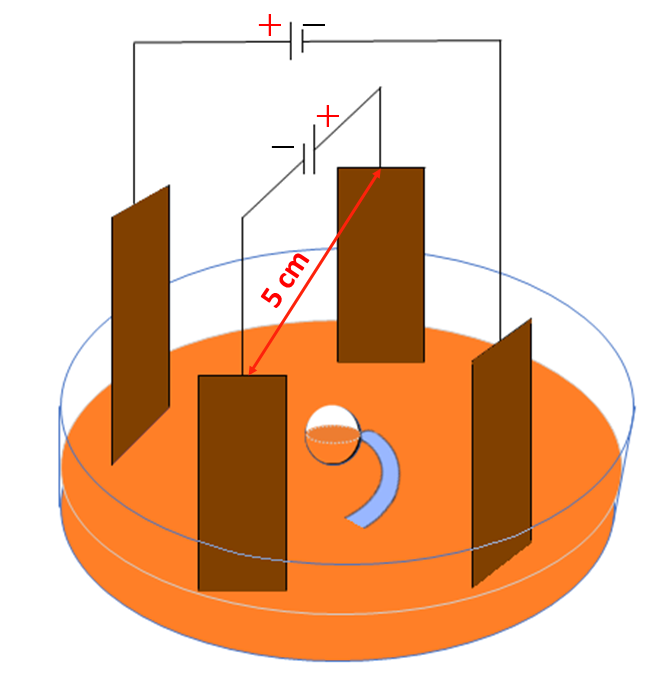
\includegraphics[scale=0.3]{expt_setup.png}
%    \caption{Schematic diagram of the experimental system: The positions of two pairs of field electrodes with respect to the glass bead are shown schematically (not to scale).}
%    \label{fig:expt_setup}
%\end{figure}

Images of the reaction medium are recorded using a CCD camera at every $30 s$ interval for a duration of $1-2$ hours. Even though the results contains only the unpinning of a spiral pinned to spherical bead, a comparative study with a spiral pinned to a cylindrical rod is included in the appendix (see appendix).
Also this article is restricted to the study of co-rotating CPEF and spiral.
%(The case of clockwise rotating spiral is included in the appendix).

\vspace{5pt}
\hrule
\vspace{5pt}

From a mathematical point of view, the dynamical features of the BZ reaction can be described using Oregonator model. 

\begin{equation}\label{E_uoregonator}
\frac{\partial u}{\partial t}=\frac{1}{\epsilon}(u(1-u)-\frac{fv(u-q)}{u+q})
+D_{u}\nabla^2u+M_{u}(\vec{E} \cdot \nabla u)
\end{equation}
\begin{equation}\label{E_voregonator}
\frac{\partial v}{\partial t}=u-v+D_{v}\nabla^2v+M_{v}(\vec{E} \cdot \nabla v).
\end{equation}

Here, $u$ is the activator variable and $v$ is the inhibitor variable (corresponding to the rescaled concentrations of [HBrO2] and the catalyst, respectively). $\vec{E} = E_{0} sin(\frac{2\pi t}{T})\hat{x} + E_{0} cos(\frac{2\pi t}{T})\hat{y}$ is the circularly polarized electric field. The electric field is added as advection an term for both the variables $u$ and $v$. 

The model parameters are $q = 0.002$, $f = 1.4$ and $\epsilon=0.04$. The diffusion coefficients are $D_{u}=1.0$ and $D_{v}=0.6$. $M_{u}=1.0$ and $M_{v}=-2.0$ are the ionic mobilities of $u$ and $v$ respectively. The computation domain of size $300 \times 300$ is discretized into grids of uniform size $dx=dy=0.1$ (s.u) in space. The explicit forward euler method with a timestep, $dt=0.0001$ is used to study the time evolution. No-flux boundary conditions are imposed both on the domain boundary and the obstacle boundary. An obstacle of radius, $r = 10$ s.u, is created at the center of the domain by reducing the value of $D_{u}=0.0001$ inside the obstacle. Phase-field method is used to set no-flux boundary conditions at the obstacle boundary \cite{fenton2005modeling}. 
All the numerical results shown this paper is carried out with the two-variable Oregonator model. But in the appendix, the results obtained from a three-variable Oregonator model is compared with those obtained from the two variable model and both shows good agreement (see the Appendix).
 

\vspace{5pt}
\hrule
\vspace{5pt}

%\section{Results and Discussions}

We denote the location of the spiral tip on the obstacle by denoting its phase, $\phi_s$. The spiral phase at t = 0 s is denoted by $\phi_0$ (initial spiral phase) and the phase at the time of unpinning is $\phi_u$ (unpinning phase). $\phi_s$ is measured anti-clockwise from the positive X-axis in degree.
%To quantify the unpinning we used a physical quantity, the spiral phase $\phi_s$. $\phi_{s}$ is the phase of the spiral at any time during its rotation on the obstacle boundary measured anti-clockwise from the positive X-axis.We measured two values of $\phi_s$: one is the initial spiral phase, $\phi_0$, at t = 0 s of field initiation and the other is the unpinning phase, $\phi_u$, at the time of spiral unpinning.
The direction of spiral tip rotation ($\hat{r_t}$) can be obtained by drawing a tangent at the respective $\phi_{s}$. In experiments, $\phi_s$ is determined from the images using the software GIMP~\cite{gimp}.
Experimental images have a resolution of 0.07 mm/pixel, which gives a resolution of 6.67$^0$ in angle measurements for a bead of diameter 1.2 mm.
In simulations, the spiral tip is defined as the intersection of two contours
$u=1/2$ and $F(1/2,v) = 0$, where $F$ is given by reaction term in equation 
(\ref{E_uoregonator})\cite{barkley1991model}.

%%%%%%%%%%%%%%%%%%%%%%%%%%%%%%%%%%%%%%%%%%%%%%%%%%%%%%%%%%%%%%%%%%%%%%%%%%%%%%%%%%%%%%%%%%%%%%%%%%%%%%%%%%%%%%%%%

\begin{figure}[H]
    \centering
    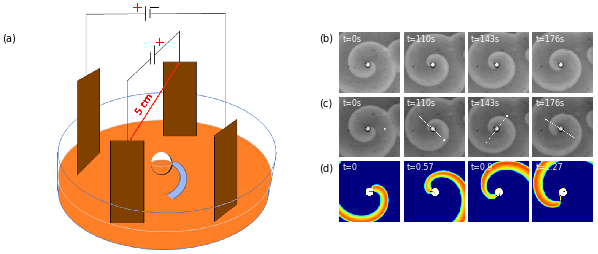
\includegraphics[scale=0.6]{Fig1.png}
    \caption{\textbf{(a) Schematic diagram of the experimental system:} The positions of two pairs of field electrodes with respect to the glass bead are shown schematically (not to scale).
    \textbf{Unpinning of an anti-clockwise rotating spiral using CPEF:}  (b) An ACW rotating spiral pinned to a spherical bead of diameter 1.2 mm in the experiment. Natural period of pinned spiral tip $T_{s} = 297 s$. (c) A CPEF of strength $E_0 \simeq 1.38 V/cm$ and period $T_{E} = 125 s$ is applied to the medium at $t=0s$. The spiral tip unpins from the obstacle and drifts away. 
    (d) An ACW rotating spiral pinned to an obstacle of diameter 1.0 s.u in the simulation with $T_{s} = 1.77$ t.u is subjected to a CPEF of strength $E_0 \simeq 0.6 $ and period $T_{E} =1.18$ t.u. The spiral tip unpins from the obstacle and drifts away.
    The arrow shows the direction of applied CPEF.}
    \label{fig:unpinning_images}
\end{figure}
 
As in the DC electric field [cite], the spiral can be unpinned with the CPEF only when the field strength E is equal to a certain threshold value $E_{th}$.
%The existence of a threshold field strength for unpinning is observed with the CPEF, in analogous with the case of a constant electric field (\cite{sutthiopad2014unpinning}).
Fig.\ref{fig:unpinning_images} gives the time sequence of field-free rotation of an ACW spiral wave, and its unpinning with a CPEF of strength $E = E_{th}$.
In experiments, an ACW spiral, pinned to an obstacle of diameter 1.2 mm, rotates with a period $T_{s} = 297 s$. The applied field have a period $T_{E} = 125 s$ and strength E = 1.38 V/cm. The ACW spiral in simulation rotates around an obstacle of diameter 1.0 s.u with a natural period $T_{s} = 1.77$ t.u. The threshold field strength in simulation is $E_{th}$ = 0.6. In both cases the spiral rotates with a lower frequency than the field ($T_{s} > T_{E}$), hence the pacing is overdrive. The ratio between the time periods of the spiral and the field rotation is denoted as the pacing ratio; $p = T_{s}/T_{E}$. In terms of $\phi_s$, $p = \theta_{E}/(\phi_{s} - \phi_{0})$, where $\theta_{E}$ is the angle covered by the field vector.
%Since both the spiral and the field co-rotates with different speed, the orientation of spiral tip with the field vector alters at each instant of their rotation depending on $T_{s}$ and $T_{E}$. We can define the quantity pacing ratio as the ratio between the time periods of the spiral and field rotation, i.e, $p = T_{s}/T_{E}$. Let $\phi_{s}$ be the phase of the spiral at any time during its rotation on the obstacle boundary measured anti-clockwise from the positive X-axis. So in terms of the phase values, p can be written  as $p = \theta_{E}/(\phi_{s} - \phi_{0})$ where, $\theta_{E}$ is the angle covered by the field and $\phi_{0}$ is the phase of the spiral at $t=0$. 

From Fig.\ref{fig:unpinning_images}~b and Fig.\ref{fig:unpinning_images}~d, it can be seen that the unpinning is initiated as the spiral start to rotate towards the cathode after passing the anode. 
In Fig.\ref{fig:unpinning_images}~b, at t = 110 s, if we mark $\hat{r_t}$ at the $\phi_{s}$ it will align parallel to the field vector $\vec{E}$. So the electric force on the spiral will be in opposite direction to $\hat{r_t}$ and hence its speed reduces. If the applied field strength is equal to $E_{th}$, this reduction in the speed of spiral rotation leads to unpinning of the tip from the obstacle. Fig.\ref{fig:acw_theory} schematically represents the above explained mechanism of spiral unpinning in a CPEF.

\begin{figure}[H]
    \centering
    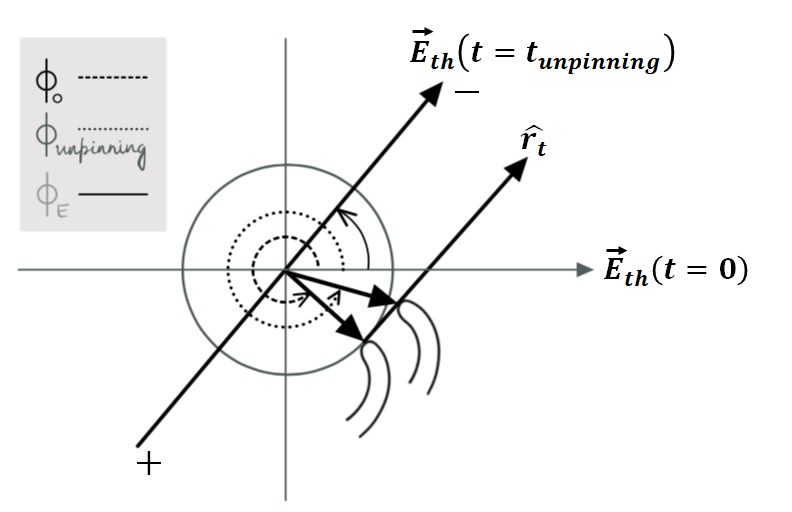
\includegraphics[width=0.8\linewidth]{cpef_theory.png}
    \caption{Schematic diagram showing the mechanism of unpinning. $\phi_{0}$ and  $\phi_{u}$ are the phase of the spiral tip at $t=0$ and at the time of unpinning respectively. $\theta_{E}$ denotes the phase of the electric field ${\vec{E}}$ and ${\hat{r}}_{t}$ is the tangential vector of spiral rotation on the obstacle boundary. All phases are measured in the anticlockwise direction from the initial direction of the $\vec{E}$ field. The wave unpins when the electric force is opposite to $\hat{r_t}$ (or when ${\vec{E}}$ and ${\hat{r}}_{t}$ are parallel to each other).
    }
    
    \label{fig:acw_theory}
\end{figure}

%%%%%%%%%%%%%%%%%%%%%%%%%%%%%%%%%%%%%%%%%%%%%%%%%%%%%%%%%%%%%%%%%%%%%%%%%%%%%%%%%%%%%%%%%%%%%%%%%%%%%%%%%%%%%%

In accordance with the mechanism at E = $E_{th}$, the unpinning for a field strength greater than $E_{th}$ must occur when the component of $\vec{E}$ along $\hat{r_t}$ reaches the critical threshold, $E_{th}$. i.e, when the scalar product of ${\vec{E}}$ and ${\hat{r}}_{t}$ is equal to or greater than $E_{th}$. This condition gives a window of possible spiral unpinning phase $\phi_{u}$ in terms of $\phi_{0}$, p, E and $E_{th}$ as in equation.\ref{eq:phiu_range}.
%\vspace{-2.5cm}
\begin{equation}
\theta_{E} - \pi + {\sin^{-1}} (\frac{E_{th}}{E})  \leq \phi_u \leq \theta_{E}-{\sin^{-1}} (\frac{E_{th}}{E}) 
\label{eq:phiu_range}
\end{equation}
where $\theta_{E}=p(\phi_s-\phi_0)$. 
For overdrive pacing with $p>1$, the unpinning phase window is given by
\begin{equation}
\frac{p \phi_0+ {\sin^{-1}}(\frac{E_{th}}{E})}{p-1}   \leq \phi_u \leq \frac{p \phi_0+\pi -{\sin^{-1}}(\frac{E_{th}}{E})}{p-1}
\label{eq:overdrive}
\end{equation}
with a width $\Delta\phi_u = \frac{\pi - 2 \sin^{-1}(\frac{E_{th}}{E})}{p-1}$.

For underdrive pacing i.e, for $p<1$, the unpinning phase window is 
\begin{equation}
\frac{\pi+ {\sin^{-1}}(\frac{E_{th}}{E})-p \phi_0}{1-p}   \leq \phi_u \leq \frac{2\pi-p \phi_0-{\sin^{-1}}(\frac{E_{th}}{E})}{1-p}
\label{eq:underdrive}
\end{equation}
The width of this window is $\Delta\phi_u = \frac{\pi - 2 \sin^{-1}(\frac{E_{th}}{E})}{1-p}$.

%%%%%%%%%%%%%%%%%%%%%%%%%%%%%%%%%%%%%%%%%%%%%%%%%%%%%%%%%%%%%%%%%%%%%%%%%%%%%%%%%%%%%%%%%%%%%%%%%%%%%%%%
%At $E_{th}$ the above conditions reduces to a single equation and the theoretical values matches well with the numerical and experimental values (Fig.\ref{fig:unpinning_Eth}). 

When E=$E_{th}$ $\phi_u = \frac{p \phi_0+ 90}{p-1}$ for overdrive pacing and $\phi_u = \frac{270-p \phi_0}{1-p}$ for underdrive pacing. Figure.\ref{fig:unpinning_Eth} shows the value of $\Delta\phi_s = \phi_u - \phi_0$ obtained in experiments and simulations. The values are in good agreement with the theoretical predictions (solid line). 

The $\phi_{u}$ values explicitly depends on the pacing ratio, p (Fig.\ref{fig:unpinning_Eth}~a) and the initial spiral phase, $\phi_{0}$ (Fig.\ref{fig:unpinning_Eth}~b-c). For example, in Fig.\ref{fig:unpinning_Eth}~a the spiral waves with $\phi_{0}$ = $225^0$ unpins with a minimum $\Delta\phi \simeq 50^0$ for $p<1$, where $\Delta\phi = \phi_{u} - \phi_{0}$ is the spiral phase difference. But the spirals with same initial phase unpins with a larger phase difference $\Delta\phi \simeq 150^0$ for $p>1$. At the same time, if we choose $\phi_{0} = 45^0$, the unpinning occurs quickly with $p>1$. 
The experiments and simulations showed that the process of unpinning is not instantaneous with the application of field, rather it requires a minimum duration of interaction between the spiral and the field. So when the field start with $\phi_{0}$ = $225^0$, the spiral experiences an opposite drag from the beginning itself. In a low pacing, it is possible to achieve the required interaction before the tip changes its orientation. But in a high pacing the orientation changes quickly and the process of unpinning comparatively delays. 
The above argument can also explain the observation of a lower $E_{th}$ value for $p<1$ (0.9 V/cm) than that for $p>1$ (1.38 V/cm).

\begin{figure}[H]
    \centering
    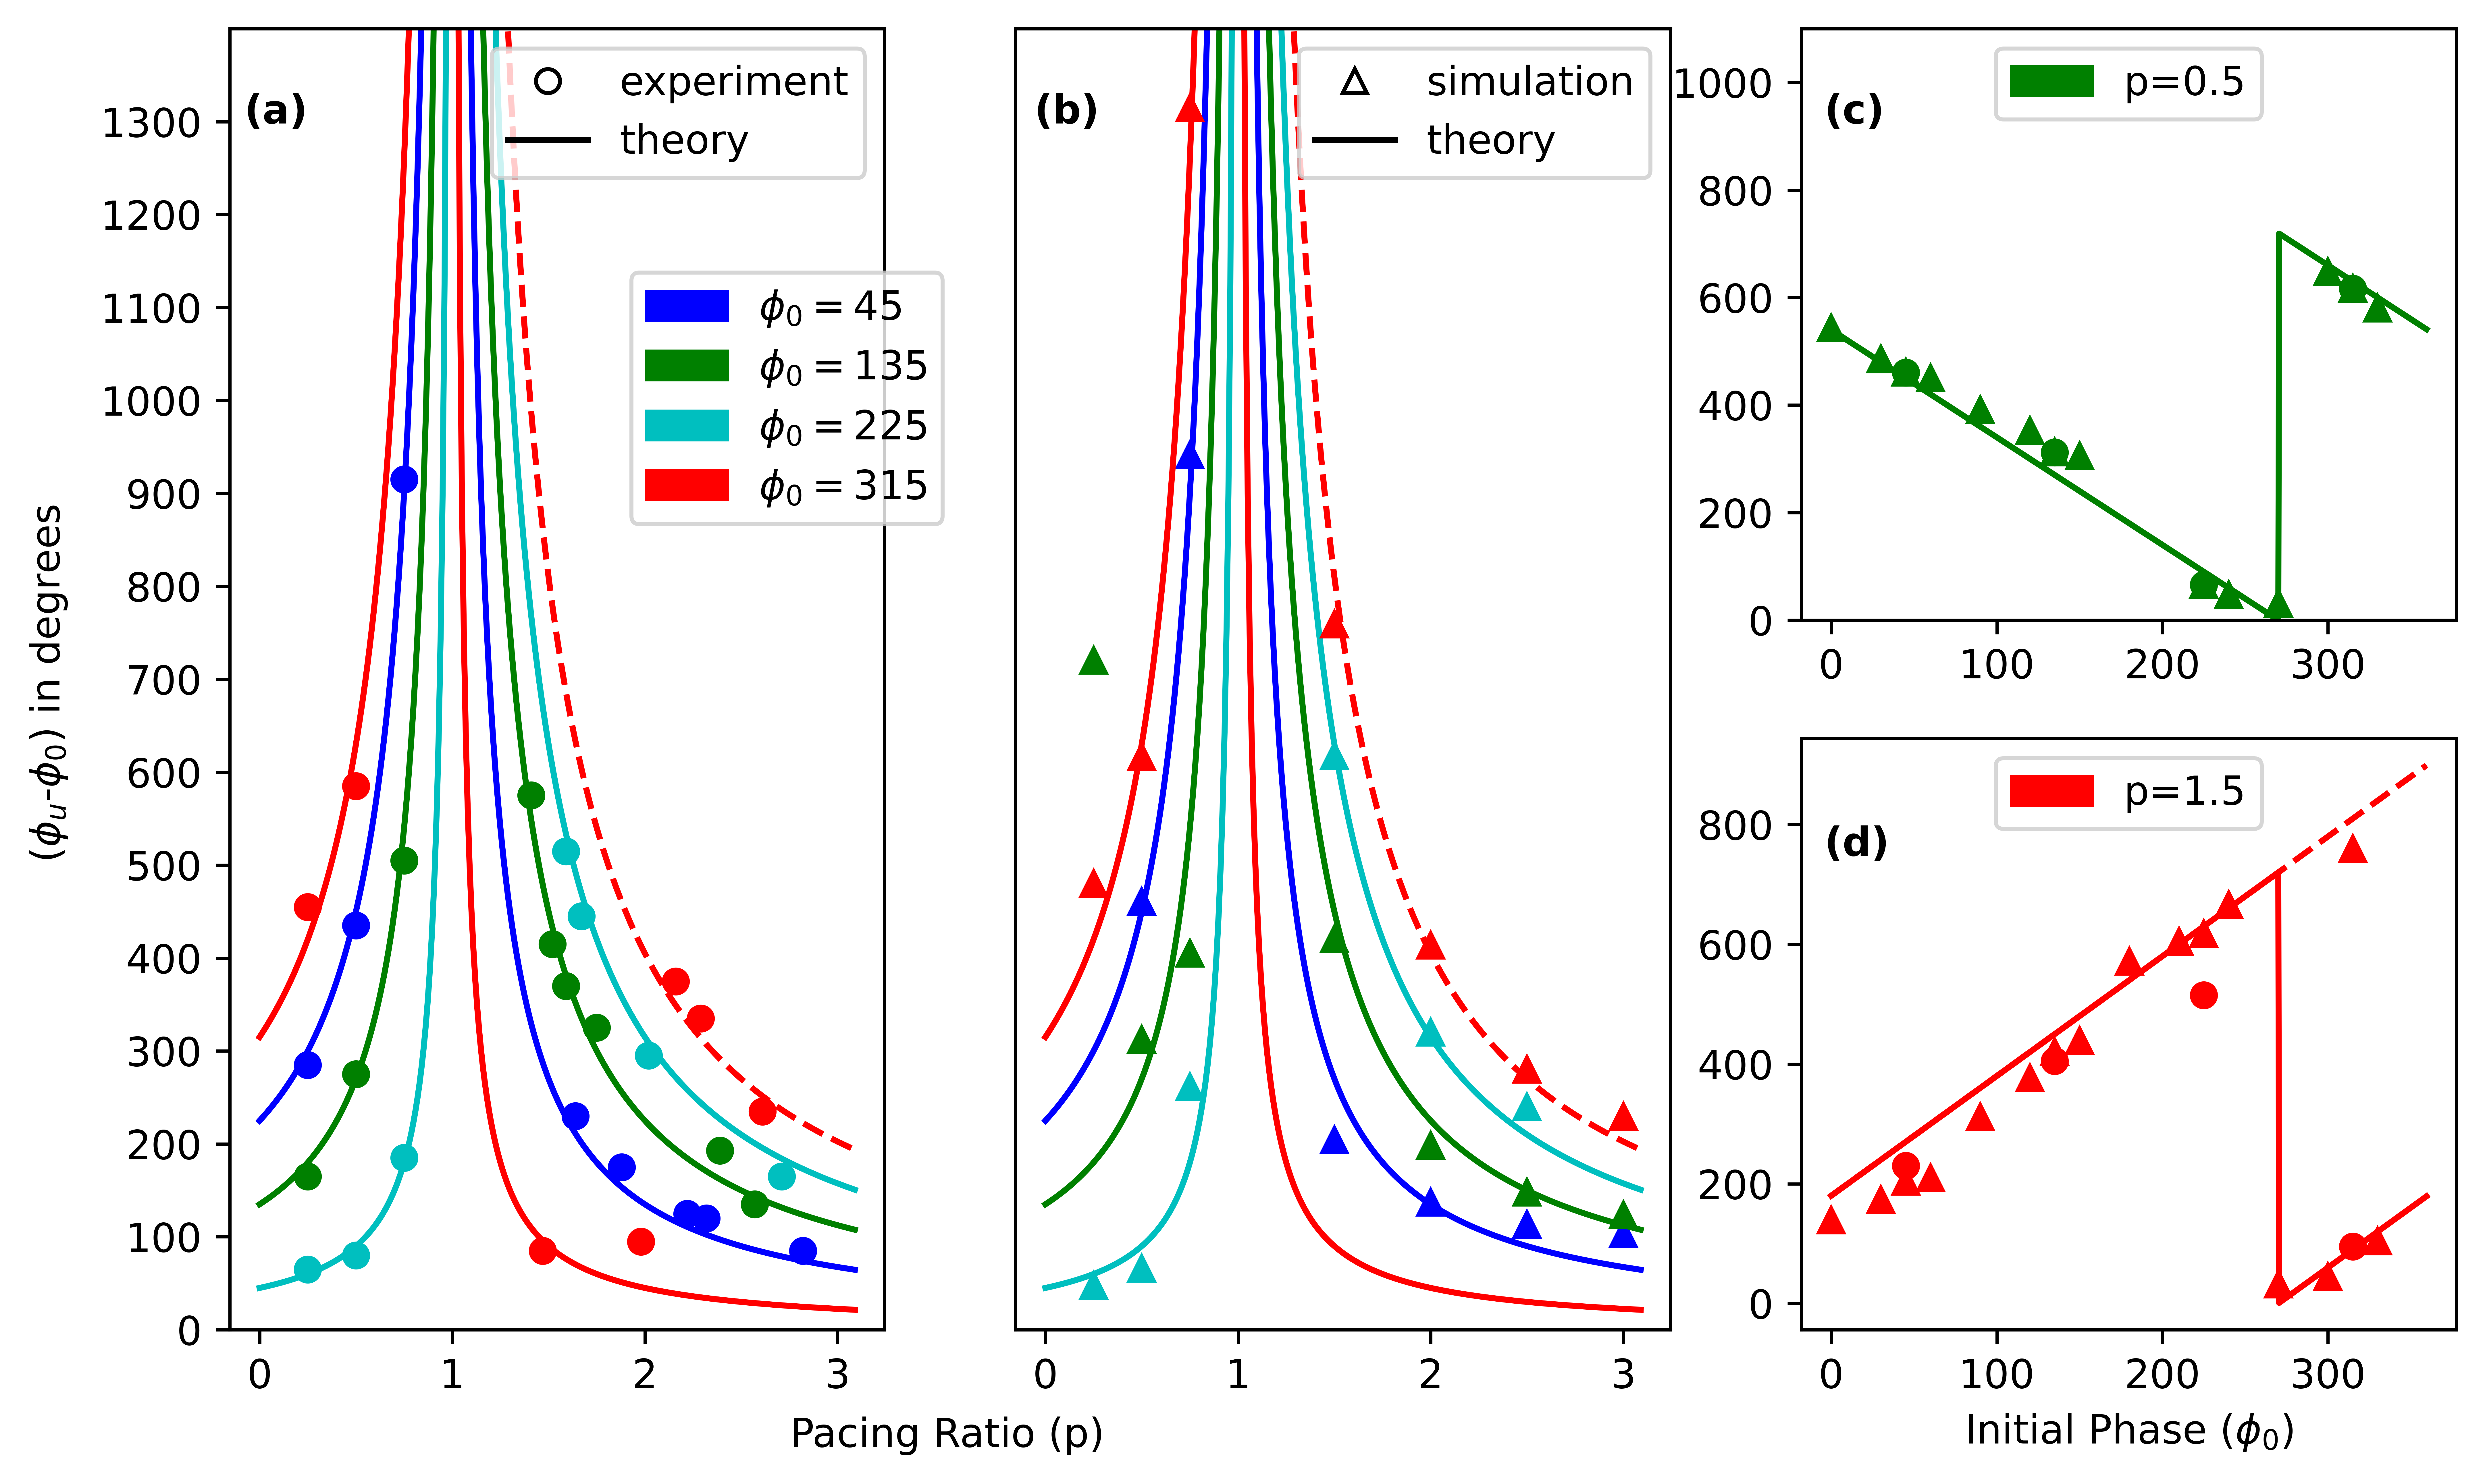
\includegraphics[scale=0.8]{Fig2.png}
    \caption{Unpinning at E=$E_{th}$: (a) For spirals having different ${\phi}_0$,  the phase difference (${\phi}_u$- ${\phi}_0$) is plotted with the pacing ratio, p. At overdrive pacing ($p>$1), the red dashed lines on the top marks the theory curve for ${\phi}_0$=$315^0$ , corresponding to the second angular positions satisfying the unpinning mechanism. The solid red line at the bottom corresponds to the first set of angular positions satisfying the unpinning mechanism for ${\phi}_0$=$315^0$.
    (b) The phase difference (${\phi}_u$- ${\phi}_0$) is plotted against ${\phi}_0$ for $p$ = 0.5 (underdrive pacing). (c) same as (b) but for $p$ = 1.5 (overdrive pacing). The condition where our unpinning condition repeats itself a second time is indicated by the dashed line. Circles and triangles represent the experiment and simulation data respectively.  
    Note: Remaining experimental data will be added later.
    }
    \label{fig:unpinning_Eth}
\end{figure}

%In Fig.\ref{fig:unpinning_Eth}~a, there are two theoretical curves for $\phi_{u}$ corresponding to $\phi_{0}$ = $315^0$. But from the equation.\ref{eq:overdrive} at E = $E_{th}$, $\phi_{u}$ can have only a single value, represented by the solid red line at the bottom. Instead, the unpinning happened at a subsequent $\phi_{s}$ after the expected $\phi_{u}$, where the condition for unpinning is satisfied (red dashed line in Fig.\ref{fig:unpinning_Eth}~a). Such a significant change occurs, most probably, when the pacing ratio is high ($p>2$). 

The variation in the unpinning phase with the initial phase is plotted in Fig.\ref{fig:unpinning_Eth}~b and Fig.\ref{fig:unpinning_Eth}~c by fixing the pacing ratio at 0.5 and 1.5 respectively. From the figures it is evident that, as $\phi_0$ increases from $0^0$ to $270^0$ $\phi_{u}$ decreases linearly for $p<1$ and increases linearly for $p>1$. At $\phi_{0} = 270^0$, there occurs a sudden raise or fall in $\Delta\phi$ value and at $\phi_{0} = 360^0$, $\Delta\phi$ resets to the value corresponding to $\phi_{0} = 0^0$. In Fig.\ref{fig:unpinning_Eth}~a, there are two theoretical curves for $\phi_{u}$ corresponding to $\phi_{0}$ = $315^0$. But from the equation.\ref{eq:overdrive} at E = $E_{th}$, $\phi_{u}$ can have only a single value, represented by the solid red line at the bottom. Instead, the unpinning happened at a subsequent $\phi_{s}$ after the expected $\phi_{u}$, where the condition for unpinning is satisfied (red dashed line in Fig.\ref{fig:unpinning_Eth}~a). The same is shown in Fig.\ref{fig:unpinning_Eth}~c as the dashed line. Such a significant change is most probable for high pacing ratios ($p>2$). 
%%%%%%%%%%%%%%%%%%%%%%%%%%%%%%%%%%%%%%%%%%%%%%%%%%%%%%%%%%%%%%%%%%%%%%%%%%%%%%%%%%%%%%%%%%%%%%%%%%%%%%%%%%%%
\begin{figure}[H]
    \centering
    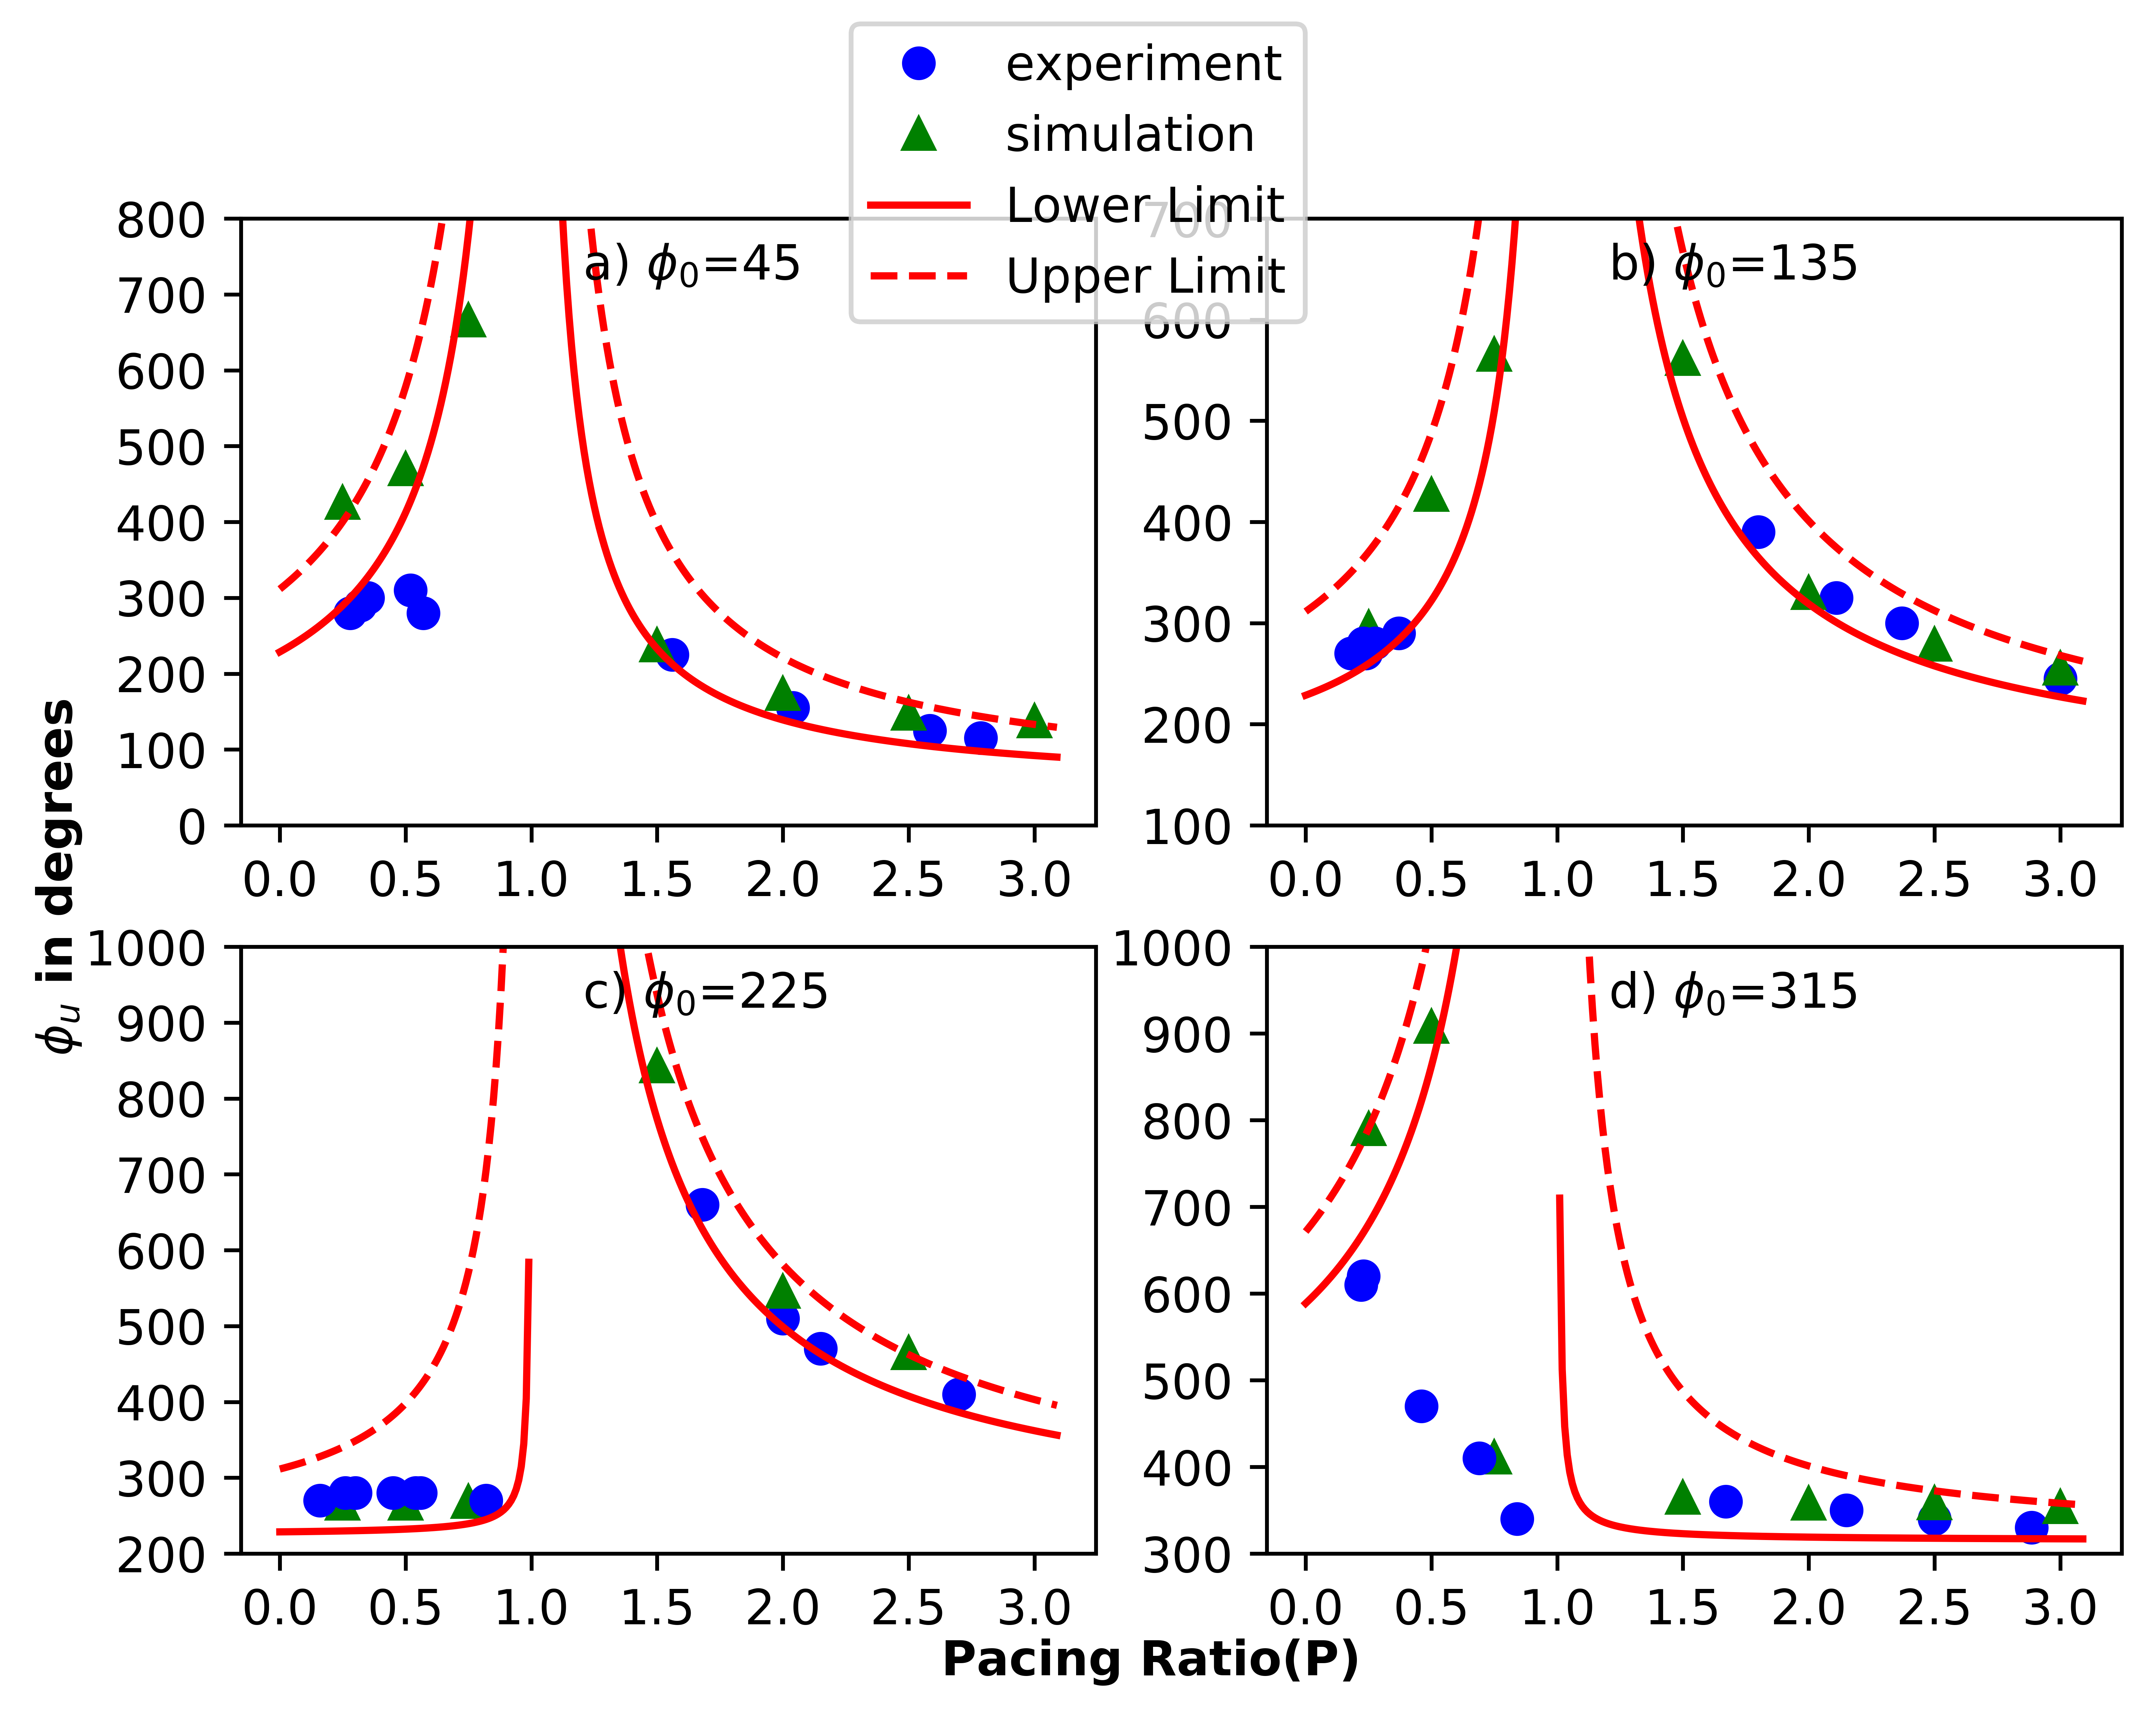
\includegraphics{E>Eth.png}
    \caption{Unpinning at $E>E_{th}$ 
    (${\sin^{-1}}{(\frac{E_{th}}{E})}=48.95^0$): Spiral waves with different ${\phi}_0$ are unpinned in a CPEF with both under-drive ($p<1$) and over-drive pacing ($p>1$). The solid bottom line represents the lower limit of the range of possible ${\phi}_u$-values given by the relation
    ${\phi}_u=(p{\phi}_0+48.95)/(p-1)$ for over-drive pacing and ${\phi}_u=(\pi-p{\phi}_0+48.59)/(1-p)$ for under-drive pacing. The upper limit of the range of possible ${\phi}_u$-values, given by the relation ${\phi}_u=(p{\phi}_0+\pi-48.95)/(p-1)$ for over-drive pacing and ${\phi}_u=(2\pi-p{\phi}_0-48.59)/(1-p)$ for under-drive pacing, are represented by the top dashed line. For ${\phi}_0 = 315^0$, the above equations must be added with $2\pi$ in order to get the positive phase values.
    Circles and triangles represent the experiment and simulation data respectively. 
    }
    \label{fig:unpinning_E>Eth}
\end{figure}

There exists an unpinning phase window corresponding to equations \ref{eq:overdrive} and \ref{eq:underdrive} for any field strength $E>E_{th}$. In Fig.\ref{fig:unpinning_E>Eth}, the solid lines corresponds to the lower limit and the dashed line corresponds to the upper limit of the window. The unpinning happens at either of these two positions which comes immediately after the required period of spiral and field interaction. Every measured $\phi_u$ values comes within these limits except a few in the case of $\phi_{0} = 315^0$. 


%%%%%%%%%%%%%%%%%%%%%%%%%%%%%%%%%%%%%%%%%%%%%%%%%%%%%%%%%%%%%%%%%%%%%%%%%%%%%%%%%%%%%%%%%%%%%%%%%%%%%%%%%%%%%
%\subsection{p=1}
If the time period of applied CPEF $T_E$ = $T_s$, the pacing ratio will be p = 1. Here the spiral and the CPEF would rotate with a fixed phase difference between them. According to the equations (\ref{eq:overdrive}) and (\ref{eq:underdrive}), p = 1 will give a $\phi_u$ which is infinity. It means that unpinning is impossible for p = 1. But in experiments and simulations we have observed unpinning with this condition, but only for a particular set of $\phi_0$ shown in figure.\ref{fig:unpinning_p1}. 
\begin{figure}[H]
    \centering
    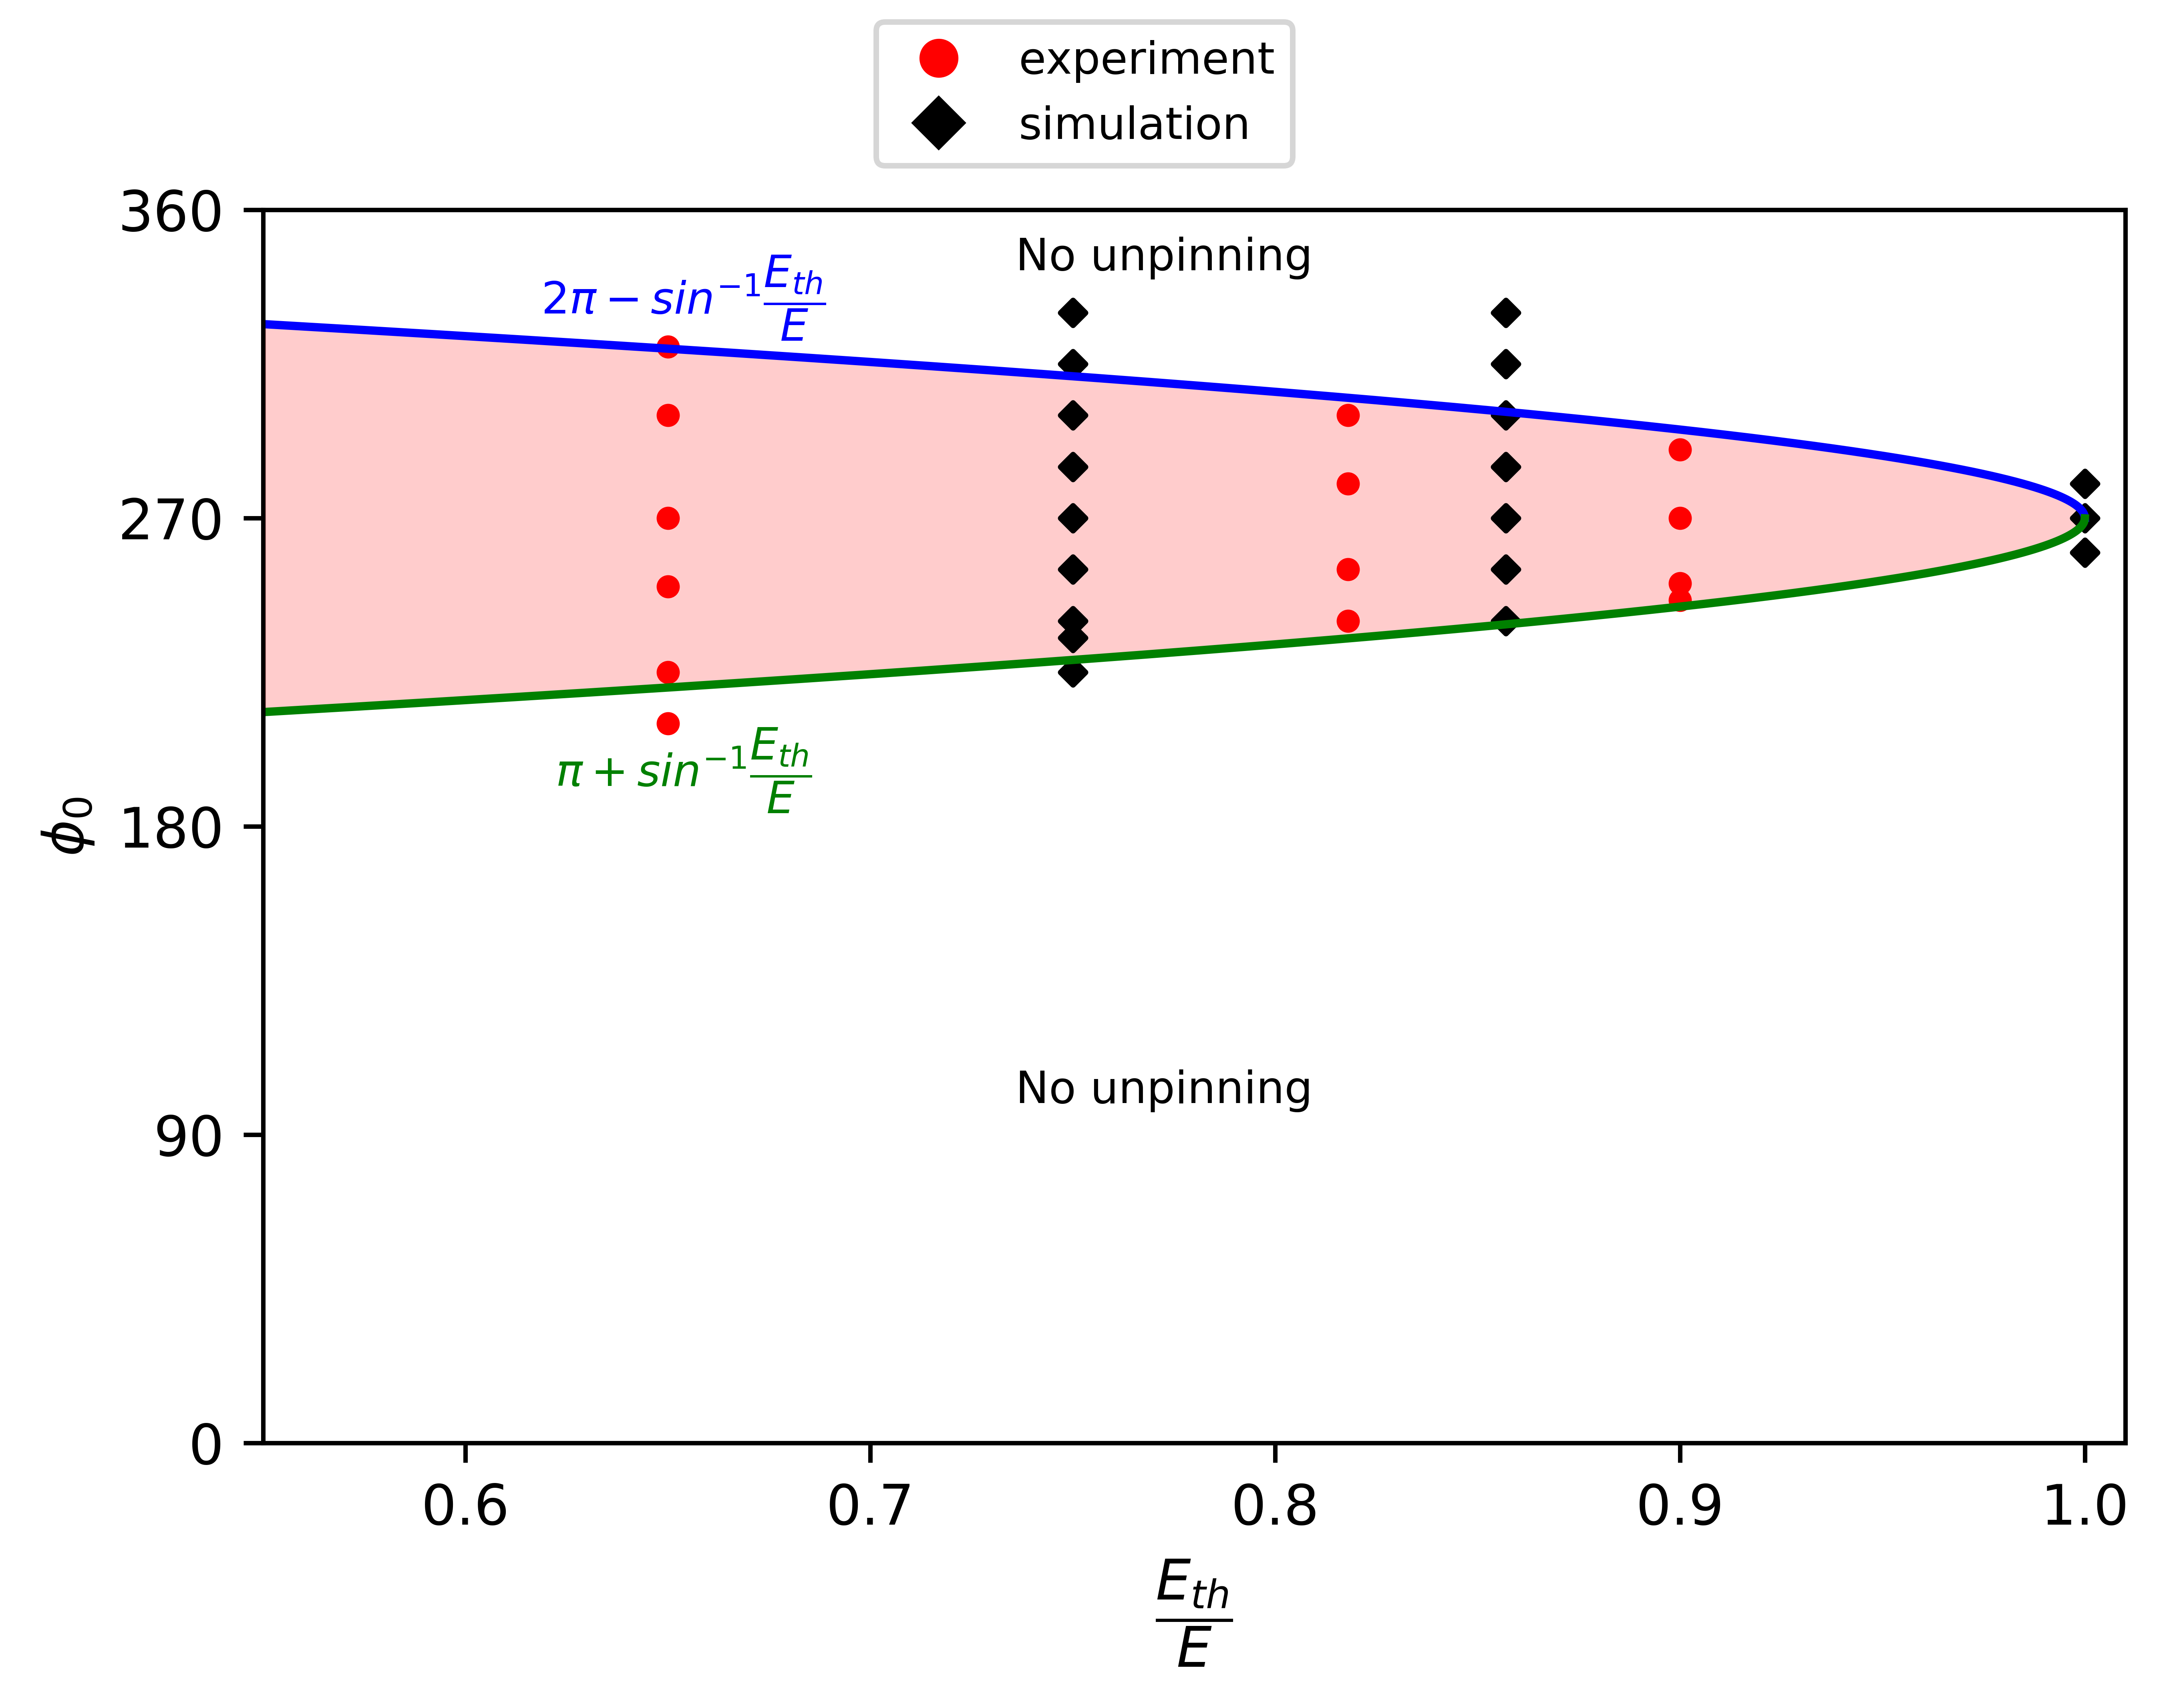
\includegraphics{p1.png}
    \caption{Unpinning of spiral wave with pacing ratio, p = 1 for different field strength: $\pi+{\sin^{-1}}{(\frac{E_{th}}{E})}$ and $2\pi-{\sin^{-1}}{(\frac{E_{th}}{E})}$ are the lower and upper limit of 
    the range of possible ${\phi}_0$-values which gives successful unpinning for p = 1. Shaded region corresponds to the cases of successful unpinning.
    Circles and diamonds represent the experiment and simulation data respectively.}
    \label{fig:unpinning_p1}
\end{figure}
For p = 1, unpinning happens only if the following condition is satisfied.
\begin{equation}
\pi+ \sin^{-1}(\frac{E_{th}}{E})  \leq \phi_0 \leq 2\pi-\sin^{-1}(\frac{E_{th}}{E})
\label{eq:p=1}
\end{equation}
This condition is reduced from the equations (\ref{eq:overdrive}) and (\ref{eq:underdrive}) by equating the numerator to zero. The width of the possible $\phi_0$-values which results in unpinning is $\Delta\phi_0 = \pi - 2 \sin^{-1}(\frac{E_{th}}{E})$. At E = $E_{th}$, $\Delta\phi_0 = 0$ and only spirals with $\phi_0 = 270^0$ unpins. For $E > E_{th}$, the unpinning is possible for a larger $\Delta\phi_0$, with a maximum value of $\pi$.  
%and it is similar to the unpinning with a DC electric field [cite DC]. 




%%%%%%%%%%%%%%%%%%%%%%%%%%%%%%%%%%%%%%%%%%%%%%%%%%%%%%%%%%%%%%%%%%%%%%%%%%%%%%%%%%%%%%%%%%%%%%%%%%%%%%%%%%%
\vspace{5pt}
\hrule
\vspace{5pt}
\section{Conclusions}

\begin{enumerate}
    \item The electric force induces a retardation in the propagation of a pinned spiral, which eventually leads to the unpinning of spiral, if the field possess a threshold amplitude. 
    
    The migration of negative bromide ions towards the anode causes the slow down in the wave speed during the cycle of spiral rotation towards the cathode.
    
    \item In general, for any field strength greater than the threshold, the unpinning occurs when the component of the electric field along the tangential direction of spiral propagation reaches the critical threshold.
    
    \item The unpinning demands a minimum interaction between the spiral and the field vector in an alignment as shown in the figure.\ref{fig:acw_theory}.
    
    \item $\phi_u$ always comes within the unpinning phase window predicted by the mathematical conditions for any field strength greater than the threshold.
   Unpinning happens at the phase which comes immediately after the required period of spiral and field interaction.
    
    \item According to the equations, $\phi_u$ depends on p, E and $\phi_0$. All these parameters fundamentally affect the interaction between the field vector and the spiral. 
    
    \item Unpinning is possible for CPEF with underdrive pacing and also for p = 1 for a particular range of $\phi_0$. To get unpinning for p = 1, the initial position of the spiral must be ahead of the anode as obtained from equation.\ref{eq:p=1}.
\end{enumerate}



The field-induced motion of $Br^-$ ions in the BZ reaction forces the core of a free spiral to drifts towards the anode. An equivalent electric force induces a retardation in the propagation of a pinned spiral, which eventually leads to its unpinning and a further drift similar to that of a free spiral. The retarding electric force can drag the spiral wave and cause unpinning only if it possess a threshold amplitude. 
In general, for any field strength greater than the threshold, the unpinning occurs when the component of the electric field along the tangential direction of spiral propagation reaches the critical threshold. This assumption leads to the deduction of conditions for the unpinning phase window.
According to which, the quantities pacing ratio, initial spiral phase and field strength provide a sensitive control over the process of unpinning. It is interesting to notice the unpinning with an electric field of lower frequency than the spiral wave in the BZ reaction. Unpinning is also possible for a unit pacing ratio with a particular set of initial phases. 

It is evident from the study that the process of unpinning is not instantaneous with the application of field, rather it requires a minimum duration of interaction between the spiral and the field; which in turn is decided by other parameters such as the pacing ratio, initial spiral phase and field strength.
The presence of mobile ions in the BZ reaction cause the excitation waves in the medium to respond in a unique manner with an applied electric field. A systematic study about this interaction will provide new insights in the control and applications of the chemical waves.



\begin{acknowledgments}

\end{acknowledgments}

\section{Author Contributions}
S.V.A, A.S, P.S, and T.K.S designed the study. S.V.A performed the experiments. P.S designed and built the experimental setup. S.P designed the numerical study as well as the computational framework. A.S performed numerical simulations. A.S, S.V.A and T.K.S formulated the theory. S.V.A and A.S collected and analysed the data with help from T.K.S. All authors helped to edit the paper. 


\appendix
\iffalse
\section{Unpinning of a CW spiral}

\begin{figure}[H]
    \centering
    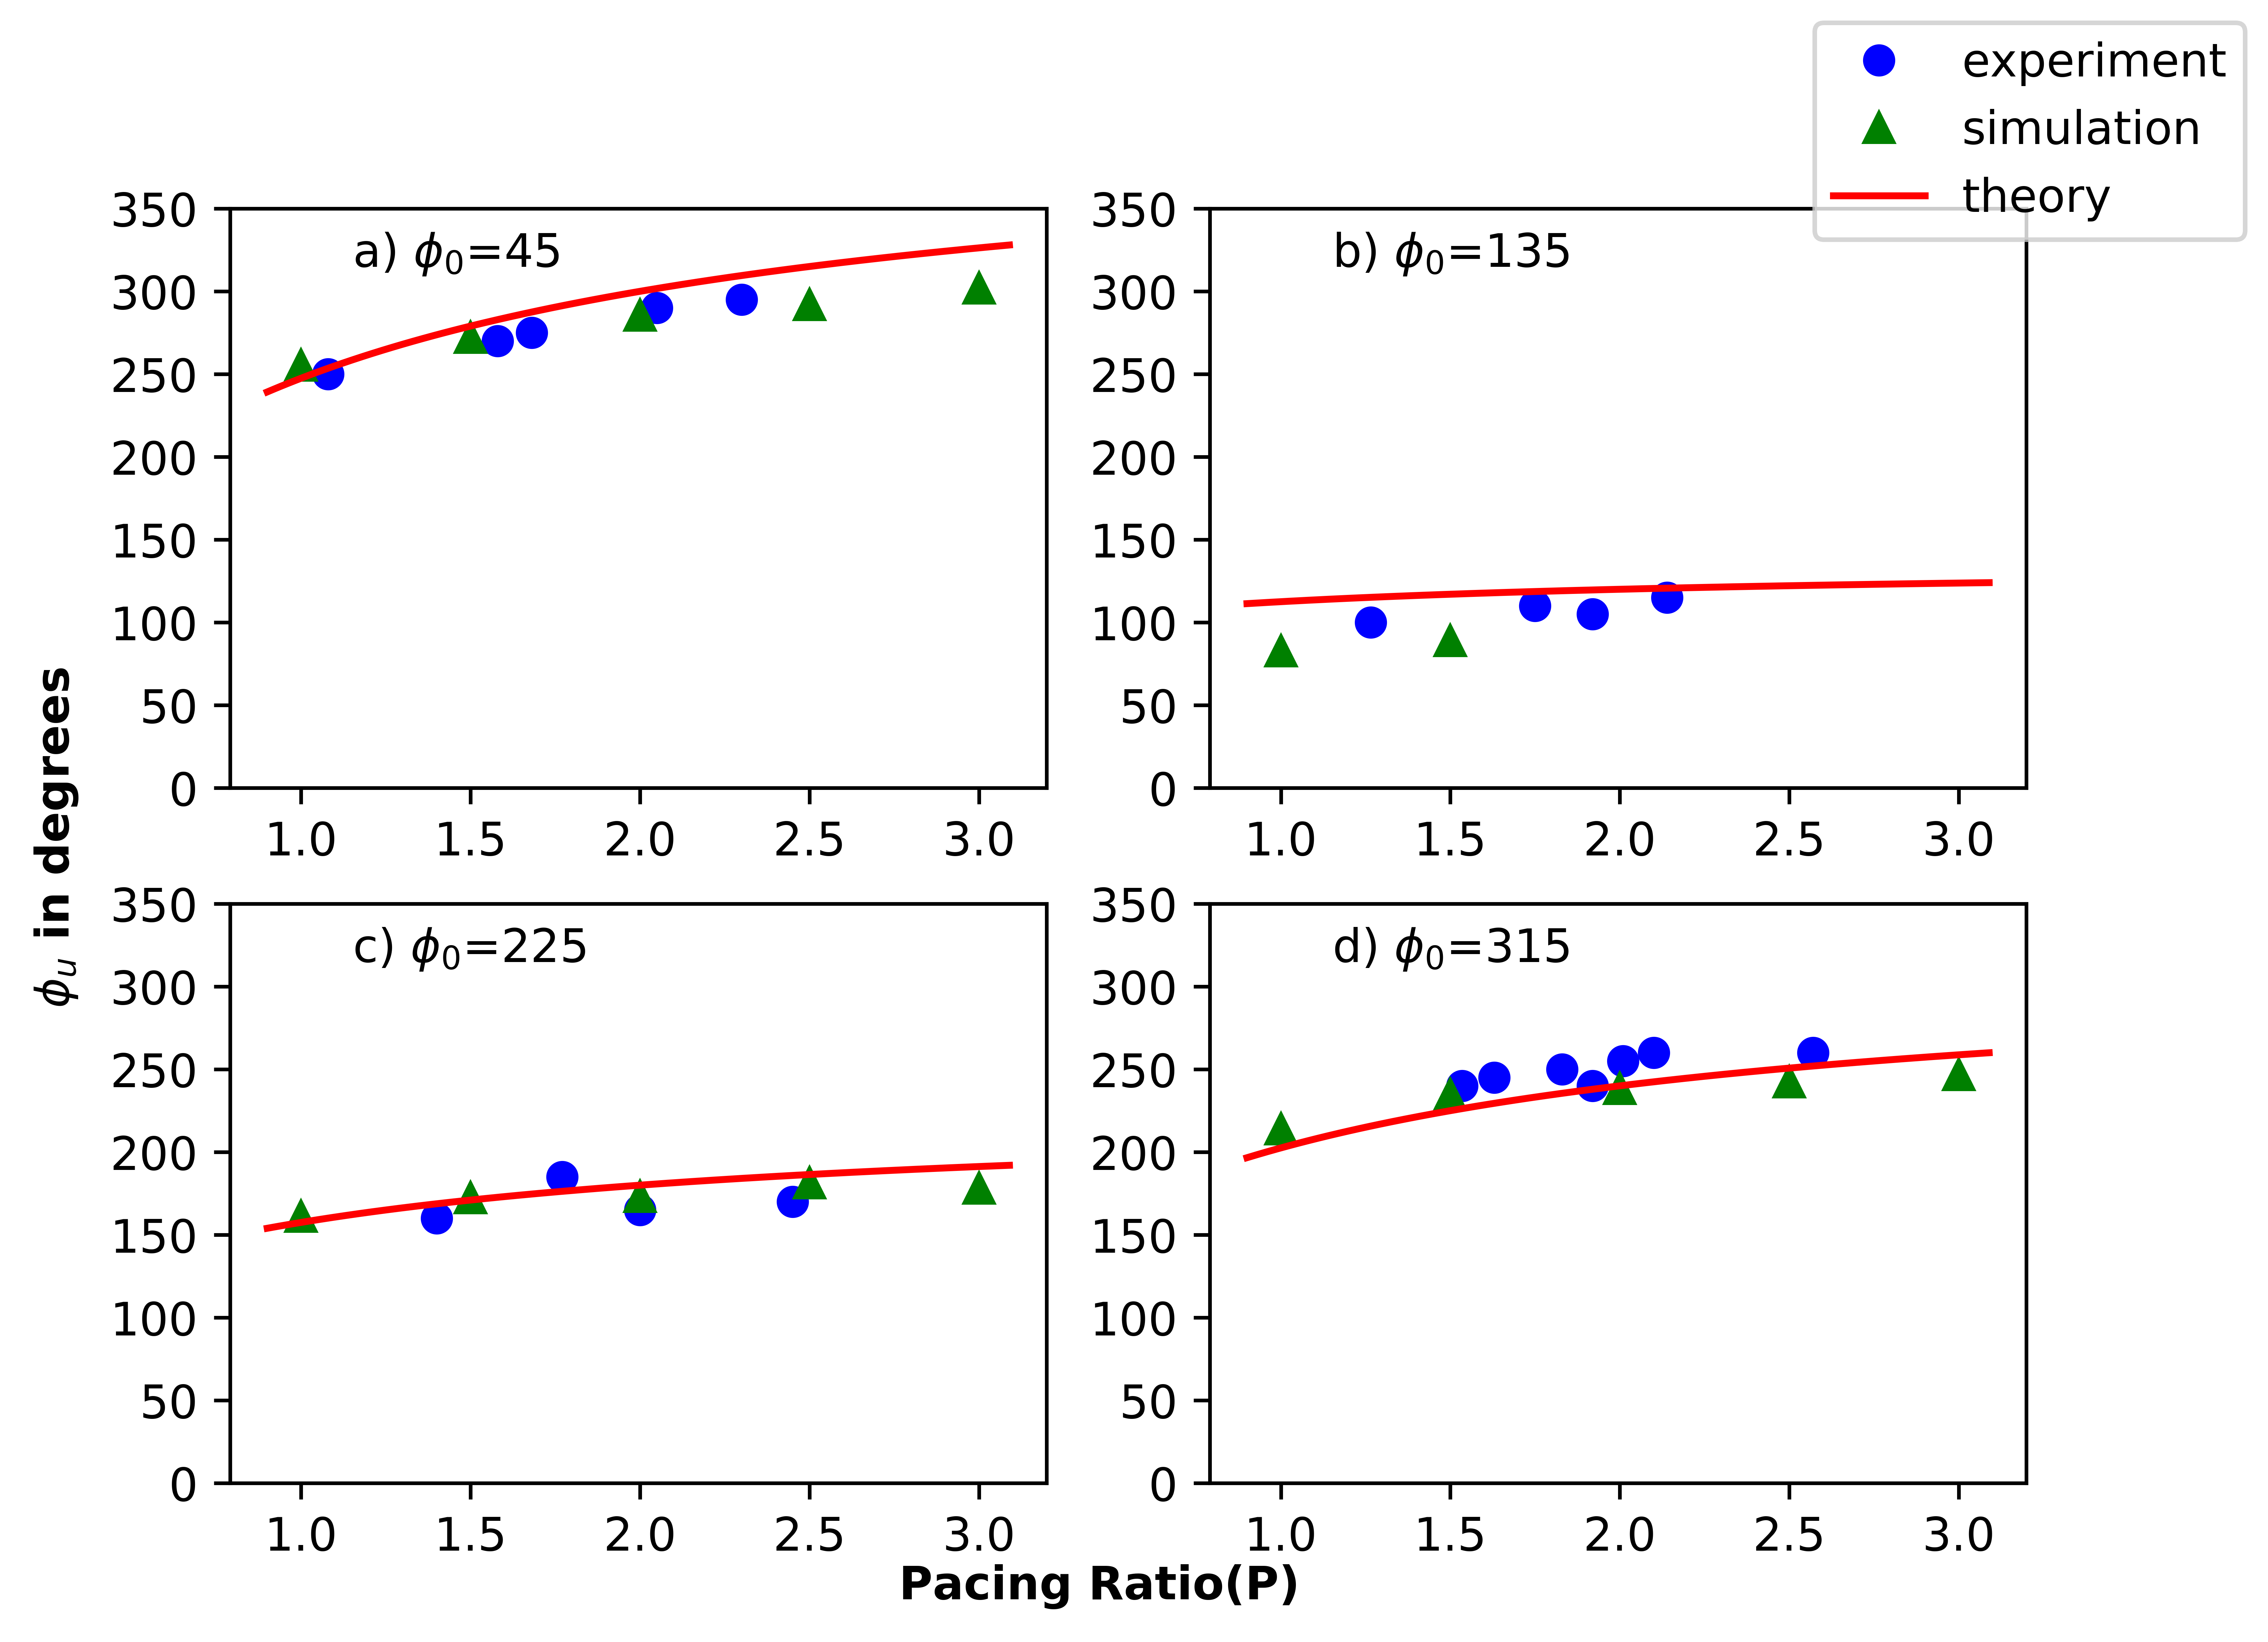
\includegraphics{appendix_cw_Eth.png}
    \caption{E=Eth}
    \label{fig:unpinning_cw}
\end{figure}
%%%%%%%%%%%%%%5 CW equation
at E=$E_{th}$
\begin{equation}
    \phi_{u} = \frac{\phi_{0}+\frac{1}{p}{\sin^{-1}} (\frac{E_{th}}{E})}{1+\frac{1}{p}}
    \label{eq:basic_eqn_cw}
\end{equation}
\centering or 
\begin{equation}
    \phi_{u} = \frac{2\pi+\phi_{0}+\frac{1}{p}{\sin^{-1}} (\frac{E_{th}}{E})}{1+\frac{1}{p}}
    \label{eq:basic_eqn_cw}
\end{equation}
\fi


%%%%%%%%%%%%%%%Comparison
\section{Comparison between numerical models and between pinning obstacles of different geometry}

\begin{figure}[H]
    \centering
    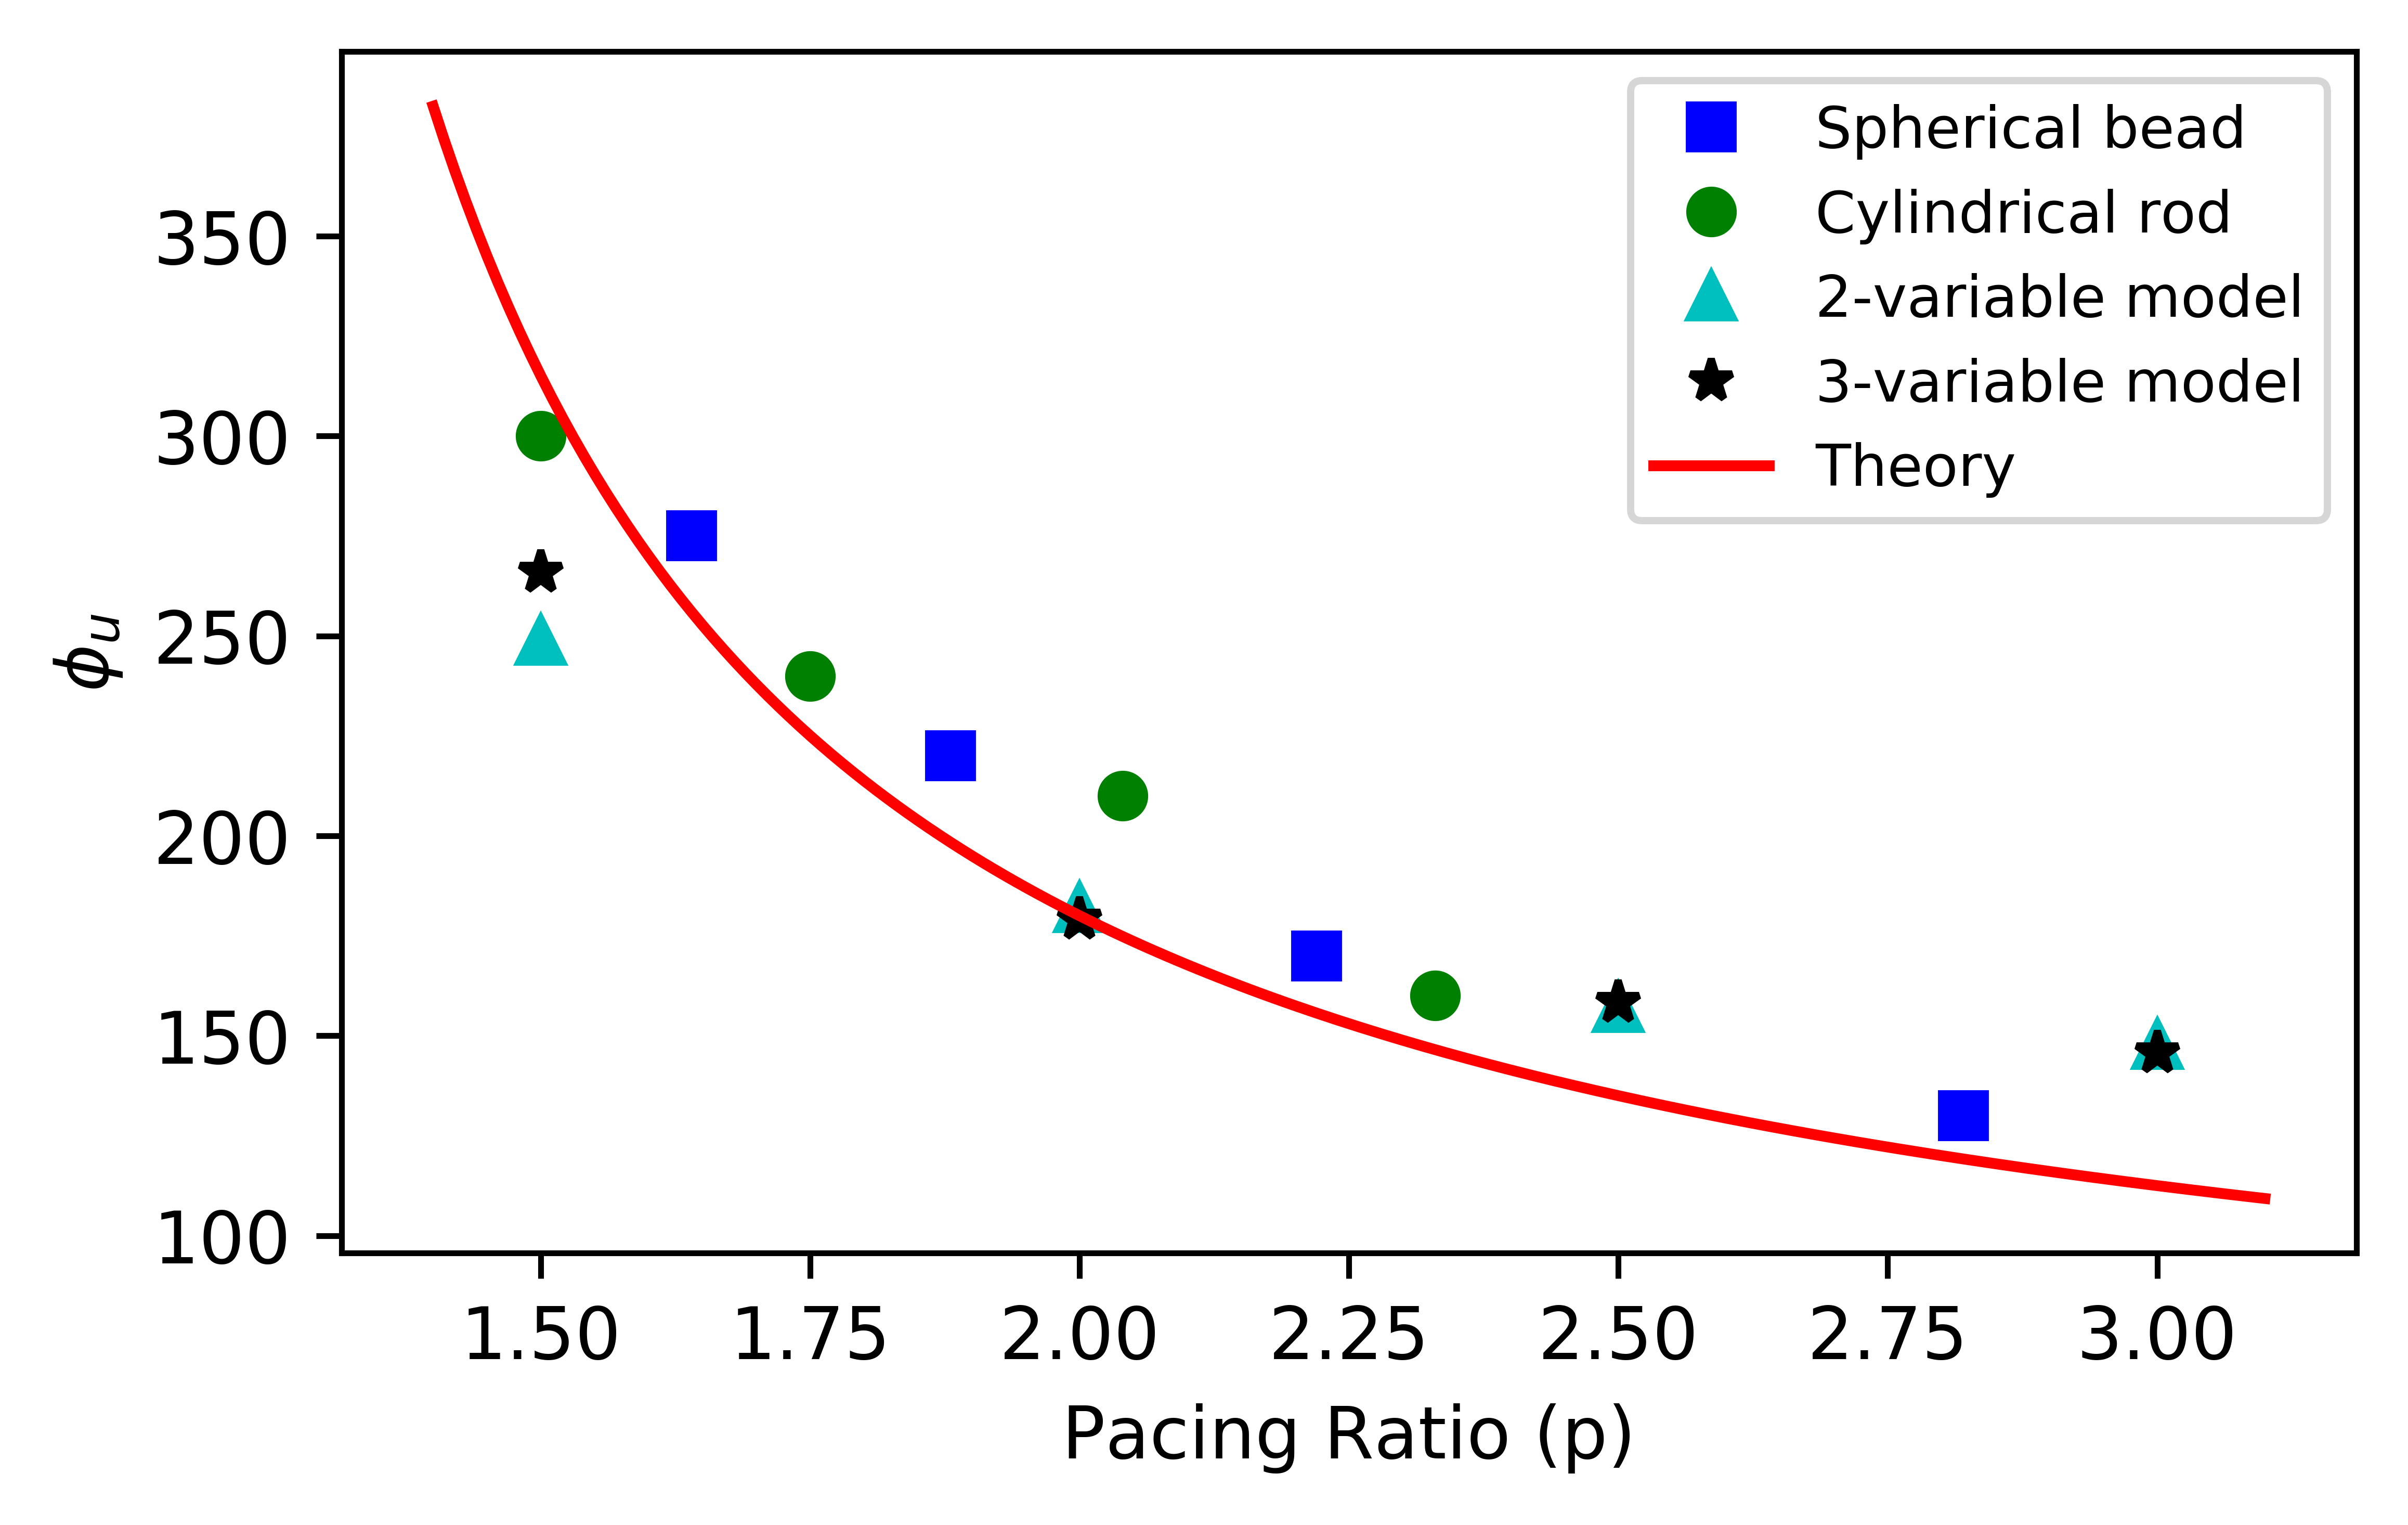
\includegraphics{appendix_23oregonator_beadrod.png}
    \caption{Caption}
    \label{fig:unpinning_comparison}
\end{figure}


\nocite{*}

\bibliography{}% Produces the bibliography via BibTeX.

\end{document}
%
% ****** End of file apssamp.tex ******

\subsection{Overdrive pacing}

\begin{equation}
\frac{p \phi_0+ {\sin^{-1}}(\frac{E_{th}}{E})}{p-1}   \leq \phi_u \leq \frac{p \phi_0+\pi -{\sin^{-1}}(\frac{E_{th}}{E})}{p-1}
\end{equation}

\subsection{ Underdrive pacing}

\begin{equation}
\frac{\pi+ {\sin^{-1}}(\frac{E_{th}}{E})-p \phi_0}{1-p}   \leq \phi_u \leq \frac{2\pi-p \phi_0-{\sin^{-1}}(\frac{E_{th}}{E})}{1-p}
\end{equation}
